%%%%%%%%%%%%%%%%%%%%%%%%%%%%%%%%%%%%%%%%%%%%%%%%%%%%%%%%%%%%%%%%%%%%%%%%%%%%%%%%
%2345678901234567890123456789012345678901234567890123456789012345678901234567890
%        1         2         3         4         5         6         7         8


%\documentclass[conference]{IEEEtran}
\documentclass[conference]{ieeeconf}
\usepackage{blindtext, graphicx}
\usepackage{listings}
\lstset { %
    language=C++,
    numbers=left,
    breaklines=true,
    xleftmargin=4em,
    resetmargins=true,
    basicstyle=\footnotesize,
    numberstyle=\footnotesize,
}
\usepackage{graphicx}
\usepackage[font=small]{caption}

%Pacote para acentos [Por TIAGO]
\usepackage[utf8]{inputenc}

% Comment this line out
                                                          % if you need a4paper
%\documentclass[a4paper, 10pt, conference]{ieeeconf}      % Use this line for a4
                                                          % paper

%\IEEEoverridecommandlockouts                              % This command is only
                                                          % needed if you want to
                                                          % use the \thanks command
%\overrideIEEEmargins
% See the \addtolength command later in the file to balance the column lengths
% on the last page of the document



% The following packages can be found on http:\\www.ctan.org
%\usepackage{graphics} % for pdf, bitmapped graphics files
%\usepackage{epsfig} % for postscript graphics files
%\usepackage{mathptmx} % assumes new font selection scheme installed
%\usepackage{times} % assumes new font selection scheme installed
%\usepackage{amsmath} % assumes amsmath package installed
%\usepackage{amssymb}  % assumes amsmath package installed

\title{Prática 1 - Robótica Móvel}

%\author{ \parbox{3 in}{\centering Huibert Kwakernaak*
%         \thanks{*Use the $\backslash$thanks command to put information here}\\
%         Faculty of Electrical Engineering, Mathematics and Computer Science\\
%         University of Twente\\
%         7500 AE Enschede, The Netherlands\\
%         {\tt\small h.kwakernaak@autsubmit.com}}
%         \hspace*{ 0.5 in}
%         \parbox{3 in}{ \centering Pradeep Misra**
%         \thanks{**The footnote marks may be inserted manually}\\
%        Department of Electrical Engineering \\
%         Wright State University\\
%         Dayton, OH 45435, USA\\
%         {\tt\small pmisra@cs.wright.edu}}
%}

% author names and affiliations
% use a multiple column layout for up to three different
% affiliations
\author{
\IEEEauthorblockN{Lucas Nogueira Nóbrega, \\Mateus Antonio da Silva}
\IEEEauthorblockA{Universidade Federal da Paraíba (UFPB)\\ João Pessoa, Brasil\\ Email: lucasnnobrega@eng.ci.ufpb.br, mateus.antonio@eng.ci.ufpb.br}
}

\begin{document}

\maketitle
\thispagestyle{empty}
\pagestyle{empty}


%%%%%%%%%%%%%%%%%%%%%%%%%%%%%%%%%%%%%%%%%%%%%%%%%%%%%%%%%%%%%%%%%%%%%%%%%%%%%%%%
\begin{abstract}

O presente relatório descreve as atividades da Prática 1 realizadas na disciplina de Robótica no período letivo 2019.2. Nessa prática alguns exercícios foram realizados para o aprendizado dos alunos, envolvendo uso dos \textit{softwares} Gazebo 3D, ROS e Matlab, a fim de integrá-los e produzir resultados na observação e controle do robô TurtleBot.

\end{abstract}


%%%%%%%%%%%%%%%%%%%%%%%%%%%%%%%%%%%%%%%%%%%%%%%%%%%%%%%%%%%%%%%%%%%%%%%%%%%%%%%%
\section{Introdução}

Esta prática consiste na utilização do \textit{TurtleBot} e \textit{Gazebo} usando a teleoperação com e sem o MATLAB, na criação de obstáculos usando o MATLAB , e na conversão de um mapa em \textit{bitmap} para \textit{OcupancyGrid}. Para integrá-los e realizar as teleoperações, o ROS (\textit{Robot Operating System}) é essencial, pois contém todos os módulos referentes a abstração de hardware, controle E funcionalidades do robô, além da troca de mensagens entre o \textit{Turtle Bot} e MATLAB. 

\section{Resultados Obtidos}

\subsection{Parte 1}

Durante a aula foi possível realizar a primeira parte da prática 1 com sucesso pois foi feito o controle do robô \textit{Turtle Bot} com o teclado, usando o \textit{software} já instalado na maquina virtual. Após a configuração das variáveis de ambiente e do \textit{teleop} para controle do robô, foi possível notar um pequeno \textit{delay} na realização das manobras, porém o turtlebot respondeu perfeitamente a todos os comandos enviados. As instruções responsáveis para comandar o turtlebot pelo teclado se encontram abaixo, utilizando as próprias dependencias do ROS:

\begin{verbatim}
$ roslaunch turtlebot_teleop 
keyboard_teleop.launch
\end{verbatim}

Já as instruções para iniciar o Gazebo pelo terminal são:

\begin{verbatim}
$ roslaunch turtlebot_gazebo 
turtlebot_mw_empty_world.launch
\end{verbatim}


\subsection{Parte 2}

A teleoperação com o MATLAB se mostrou interessante, pois o controle foi realizado com dois notebooks, mostrando o controle do \textit{Turtle Bot} no Gazebo a distância. Com as configurações de odometria e do laser scan feitas no Matlab, foi possível observar não só a visão do robô através de um gráfico, como sua trajetória baseada nos comandos enviados pelo teclado. A visão do robô é atualizada de acordo com o posicionamento da sua câmera e com isso pode ser controlado mesmo sem a visualização do cenário 3D. Ver figura \ref{fig:twoComputers}.

\begin{figure}[!htb]
\centering
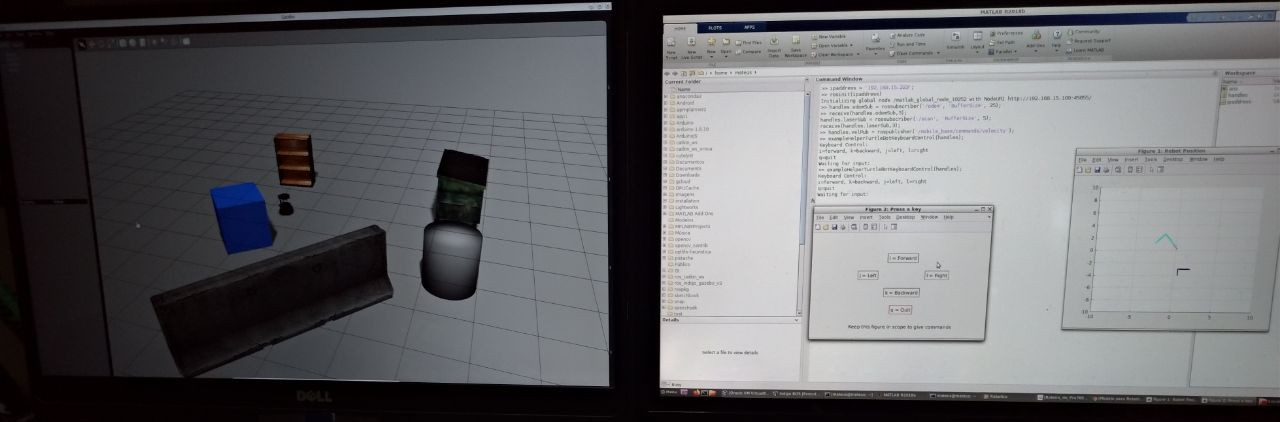
\includegraphics[width=5.5cm]{twoComputers.jpg}
\caption{Integração MatlabxGazebo entre dois computadores}
\label{fig:twoComputers}
\end{figure}
 
\subsection{Parte 3}

Também utilizando dois computadores, foi realizado a criação de obstáculos utilizando a comunicação entre o MATLAB e Gazebo. Estes obstáculos consistiram em muros, esferas , entre outros objetos no qual o robô pode detectar usando os sensores embutidos nele. Na figura \ref{fig:GazeboWalls} pode observar o comportamento da prática.

\begin{figure}[!htb]
\centering
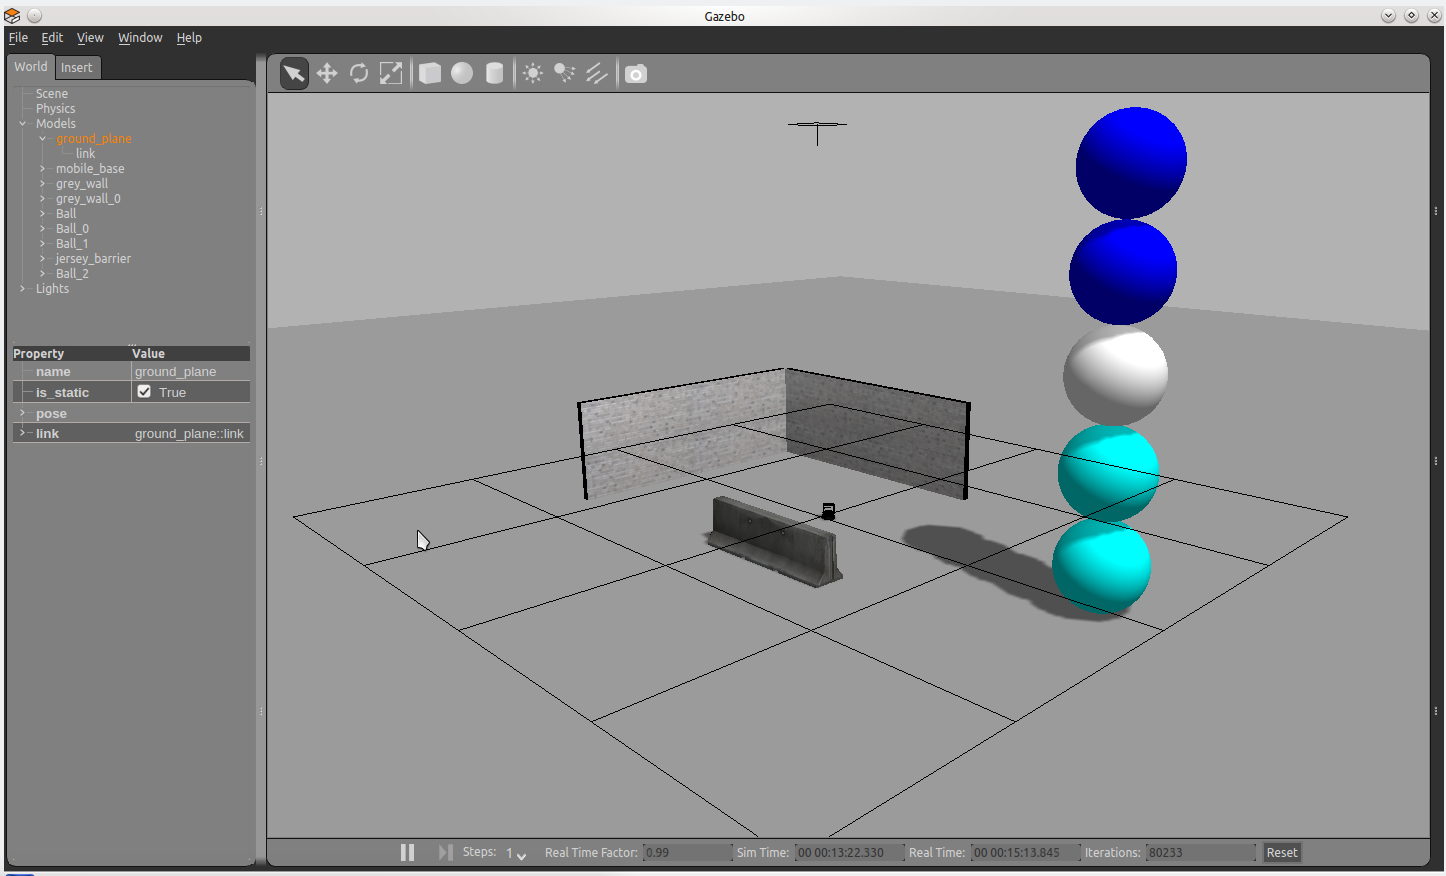
\includegraphics[width=5.5cm]{GazeboWalls.png}
\caption{Gazebo com obstáculos criados pelo MATLAB}
\label{fig:GazeboWalls}
\end{figure}

\newpage

\subsection{Parte 4}

A criação do mapa foi proveniente da imagem na prática, em que tiramos uma foto em 450 por 360 \textit{pixels} e depois foi salvo em formato \textit{Bitmap}. Esta foto foi processada com as ferramentas do MATLAB para que a proporção entre os \textit{pixels} e metros ficassem na escala correta, por isso foi escolhido que a resolução fosse de 50, como mostra na figura \ref{fig:ocupancyGrid}. Após esse algorítimo geramos o seguinte \textit{Ocupancy Grid}.

\begin{figure}[!htb]
\centering
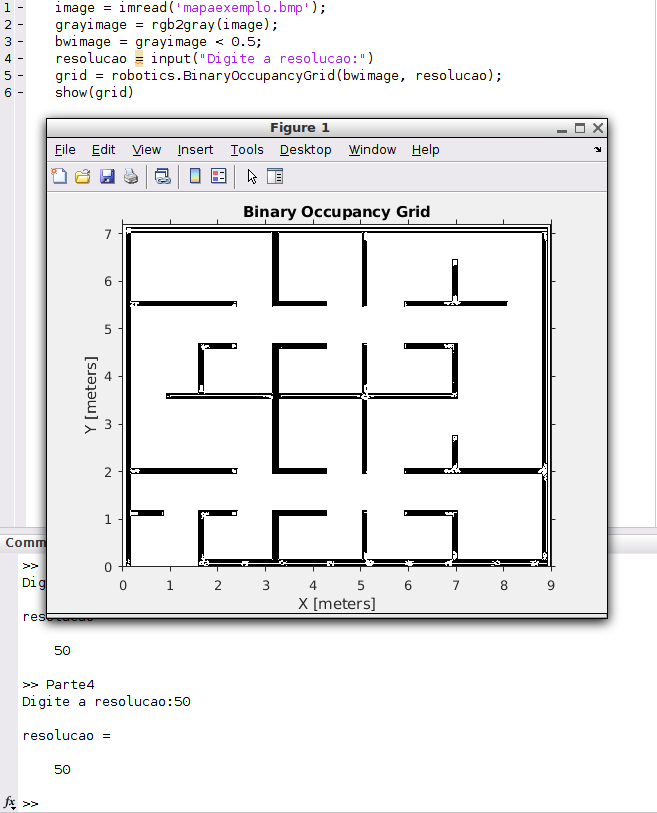
\includegraphics[width=3.5cm]{mapa.png}
\caption{\textit{Ocupancy Grid}}
\label{fig:ocupancyGrid}
\end{figure}


\section{Discussão dos Resultados}

A primeira parte da prática aconteceu sem problemas pois todos os comandos para a teleoperação como os para iniciar o Gazebo foram realizados na máquina virtual, que se encontra devidamente configurada para \textit{download} no site do MATLAB.

A segunda parte ofereceu certas dificuldades de conexão do Matlab na máquina \textit{host} com o Gazebo na máquina virtual, porém foi superado através das devidas configurações da placa de rede maquina virtual em modo \textit{bridge} que possibilitou a comunicação da maquina virtual com um outro computador na mesma rede local. Isso nos forneceu uma paralelização das atividades e do processamento de dados, o que tornou a prática mais rápida.

Foi esperado que a terceira parte acontecesse mais rápida já que o processamento computacional era dividido entre duas máquinas. Porém ainda tivemos que esperar para que o primeiro objeto da figura fosse renderizado. Após a primeira renderização os outros objetos eram inseridos na simulação mais rapidamente.

A criação do \textit{Ocupancy Grid} foi realizada com sucesso, considerando que tivemos que usar uma proporção correta para a converter de Bitmap.


\addtolength{\textheight}{-12cm}   % This command serves to balance the column lengths
                                  % on the last page of the document manually. It shortens
                                  % the textheight of the last page by a suitable amount.
                                  % This command does not take effect until the next page
                                  % so it should come on the page before the last. Make
                                  % sure that you do not shorten the textheight too much.

%%%%%%%%%%%%%%%%%%%%%%%%%%%%%%%%%%%%%%%%%%%%%%%%%%%%%%%%%%%%%%%%%%%%%%%%%%%%%%%%

%\bibliographystyle{IEEEtran}  
%\bibliography{IEEEexample}

\end{document}
